\chapter{Rigid motion and Lie groups}
\label{ch:rigid}

Chapter~\ref{ch:slam} wrote residuals such as $\x_k-f(\x_{k-1},\uu_k)$ and
then differentiated them, as if poses lived in a vector space. They do
not: the composition of two rotations is not their sum, and the
``average'' of two rotation matrices is not a rotation. This chapter
builds the minimal machinery that makes every later formula legitimate:
the groups $\SO3$ and $\SE3$, their Lie algebras, the exponential and
logarithm maps that move between them, and a calculus of small
perturbations that lets us write Jacobians and covariances of poses as
ordinary matrices.

The guiding idea is simple. Near any pose, the group looks like
$\R^6$; we do all our linear algebra in that local $\R^6$ and use the
exponential map to step back onto the group. Everything else is
bookkeeping, and the bookkeeping must be exact, because a sign error in a
Jacobian is the most common reason a SLAM back-end silently diverges.

\section{Rotations}

\begin{definition}{Special orthogonal group}{so3}
$\SO3=\{R\in\R^{3\times3}: R\T R=I,\ \det R=1\}$. With matrix
multiplication it is a group: closed under products and inverses
($R^{-1}=R\T$), with identity $I$. A rotation $R_{ab}$ maps coordinates
of a vector expressed in frame $b$ to its coordinates in frame $a$:
$\vect{v}_a=R_{ab}\vect{v}_b$.
\end{definition}

$\SO3$ is a smooth 3-dimensional submanifold of $\R^{9}$: nine entries
subject to six independent constraints ($R\T R=I$ is symmetric). Three
degrees of freedom, but no global parametrisation by $\R^3$ without
singularities (Euler angles have gimbal lock). We will never use a
global parametrisation; we will use \emph{local} ones around the current
estimate.

\subsection{Skew-symmetric matrices}

\begin{definition}{Hat and vee operators}{hat}
For $\vect{a}=(a_1,a_2,a_3)\T\in\R^3$,
\[
\hatop{\vect{a}}=\begin{pmatrix}0&-a_3&a_2\\a_3&0&-a_1\\-a_2&a_1&0
\end{pmatrix},
\]
and $\veeop{(\cdot)}$ is its inverse on skew-symmetric matrices.
\end{definition}

\begin{lemma}{Identities of the hat operator}{hatid}
For $\vect{a},\vect{b}\in\R^3$ and $R\in\SO3$:
\begin{enumerate}[label=(\roman*),nosep]
\item $\hatop{\vect{a}}\vect{b}=\vect{a}\times\vect{b}$ and
  $(\hatop{\vect{a}})\T=-\hatop{\vect{a}}$;
\item $(\hatop{\vect{a}})^2=\vect{a}\vect{a}\T-\norm{\vect{a}}^2I$;
\item $(\hatop{\vect{a}})^3=-\norm{\vect{a}}^2\,\hatop{\vect{a}}$;
\item $R(\vect{a}\times\vect{b})=(R\vect{a})\times(R\vect{b})$;
\item $R\,\hatop{\vect{a}}\,R\T=\hatop{(R\vect{a})}$.
\end{enumerate}
\end{lemma}

\begin{proof}
(i) is a direct check of the definition. (ii) For any $\vect{b}$,
$\vect{a}\times(\vect{a}\times\vect{b})=\vect{a}(\vect{a}\T\vect{b})-
\norm{\vect{a}}^2\vect{b}$ (the ``BAC--CAB'' rule). (iii) Multiply (ii)
on the left by $\hatop{\vect{a}}$ and use $\hatop{\vect{a}}\vect{a}=
\vect{a}\times\vect{a}=\vect{0}$. (iv) For any $\vect{w}$, the scalar
triple product gives
$\vect{w}\T R(\vect{a}\times\vect{b})=(R\T\vect{w})\T(\vect{a}\times
\vect{b})=\det[R\T\vect{w},\vect{a},\vect{b}]$. Since
$[R\T\vect{w},\vect{a},\vect{b}]=R\T[\vect{w},R\vect{a},R\vect{b}]$ and
$\det R\T=1$, this equals $\det[\vect{w},R\vect{a},R\vect{b}]=
\vect{w}\T\bigl((R\vect{a})\times(R\vect{b})\bigr)$. As $\vect{w}$ is
arbitrary, (iv) follows. (v) For any $\vect{b}$, by (iv) applied to
$\vect{a}$ and $R\T\vect{b}$:
$R\,\hatop{\vect{a}}R\T\vect{b}=R(\vect{a}\times R\T\vect{b})=
(R\vect{a})\times\vect{b}$.
\end{proof}

Note that (iv) uses $\det R=+1$: a reflection reverses cross products.
This is one of many places where the ``special'' in special orthogonal
matters.

\subsection{The Lie algebra}

\begin{proposition}{Tangent space at the identity}{tangent}
If $t\mapsto R(t)$ is a differentiable curve in $\SO3$, then
$R(t)\T\dot R(t)$ and $\dot R(t)R(t)\T$ are skew-symmetric for every $t$.
In particular the tangent space of $\SO3$ at $I$ is contained in
$\so3=\{\hatop{\vect{a}}:\vect{a}\in\R^3\}$, the space of
skew-symmetric matrices.
\end{proposition}

\begin{proof}
Differentiate $R\T R=I$: $\dot R\T R+R\T\dot R=0$, i.e.\
$(R\T\dot R)\T=-R\T\dot R$. Likewise from $RR\T=I$.
\end{proof}

The two skew matrices have names: $\hatop{\bomega_b}=R\T\dot R$ gives the
\emph{body} angular velocity (the one a gyroscope measures, Chapter~12),
and $\hatop{\bomega_a}=\dot RR\T$ the \emph{spatial} one; by
\cref{lem:hatid}(v), $\bomega_a=R\bomega_b$. The converse inclusion,
that every skew matrix is a tangent vector, follows from the next
section: $t\mapsto\exp(t\hatop{\vect{a}})$ is a curve in $\SO3$ with
velocity $\hatop{\vect{a}}$ at $t=0$. The vector space $\so3$, equipped
with the commutator $[A,B]=AB-BA$, is the \emph{Lie algebra} of $\SO3$.
Through hat and vee we identify it with $\R^3$, and then the
commutator is just the cross product:
$[\hatop{\vect{a}},\hatop{\vect{b}}]=\hatop{(\vect{a}\times\vect{b})}$.

\section{The exponential and the logarithm}

\begin{theorem}{Rodrigues' formula}{rodrigues}
For $\bphi\in\R^3$ with $\theta=\norm{\bphi}\neq0$, the matrix
exponential of $\hatop{\bphi}$ is
\begin{equation}\label{eq:rodrigues}
\Exp(\bphi)\coloneqq\exp(\hatop{\bphi})
=I+\frac{\sin\theta}{\theta}\hatop{\bphi}
 +\frac{1-\cos\theta}{\theta^2}(\hatop{\bphi})^2,
\end{equation}
and $\Exp(\vect{0})=I$. Moreover $\Exp(\bphi)\in\SO3$.
\end{theorem}

\begin{proof}
Write $\bphi=\theta\vect{a}$ with $\norm{\vect{a}}=1$ and $K=
\hatop{\vect{a}}$. By \cref{lem:hatid}(iii), $K^3=-K$, hence by induction
$K^{2m+1}=(-1)^mK$ and $K^{2m+2}=(-1)^mK^2$ for $m\ge0$. Splitting the
(absolutely convergent) exponential series into odd and even powers,
\[
\exp(\theta K)=I+\Bigl(\sum_{m\ge0}\frac{(-1)^m\theta^{2m+1}}{(2m+1)!}
\Bigr)K+\Bigl(\sum_{m\ge0}\frac{(-1)^m\theta^{2m+2}}{(2m+2)!}\Bigr)K^2
=I+\sin\theta\,K+(1-\cos\theta)K^2 .
\]
Substituting $K=\hatop{\bphi}/\theta$ gives \eqref{eq:rodrigues}. For
membership in $\SO3$: $\exp(S)\T=\exp(S\T)=\exp(-S)=\exp(S)^{-1}$ for
skew $S$, and $\det\exp(S)=e^{\tr S}=e^0=1$.
\end{proof}

\begin{inwords}
$\Exp(\theta\vect{a})$ is the rotation by angle $\theta$ about the unit
axis $\vect{a}$. Indeed $K\vect{a}=\vect{0}$, so the axis is fixed; and
for a unit $\vect{b}\perp\vect{a}$, $K\vect{b}=\vect{a}\times\vect{b}$ and
$K^2\vect{b}=-\vect{b}$, so $\Exp(\theta\vect{a})\vect{b}=\cos\theta\,
\vect{b}+\sin\theta\,(\vect{a}\times\vect{b})$: a right-handed rotation
by $\theta$ in the plane orthogonal to $\vect{a}$. The vector $\bphi$ is
the familiar ``axis--angle'' or \emph{rotation vector}.
\end{inwords}

\begin{proposition}{Logarithm of a rotation}{log}
Every $R\in\SO3$ equals $\Exp(\bphi)$ for some $\bphi$ with
$\norm{\bphi}\le\pi$, and $\theta=\norm{\bphi}$ satisfies
\begin{equation}\label{eq:trace}
\cos\theta=\tfrac12(\tr R-1).
\end{equation}
If $0<\theta<\pi$, $\bphi$ is unique and
\begin{equation}\label{eq:log}
\Log(R)\coloneqq\bphi=\frac{\theta}{2\sin\theta}\,\veeop{(R-R\T)} .
\end{equation}
If $\theta=0$ then $R=I$ and $\bphi=\vect{0}$. If $\theta=\pi$ then
$R=2\vect{a}\vect{a}\T-I$ and $\bphi=\pm\pi\vect{a}$ (both are valid).
\end{proposition}

\begin{proof}
\emph{Existence.} $R$ has the eigenvalue $1$: since $\det R=1$ and $3$ is
odd,
\[
\det(R-I)=\det\bigl(R(I-R\T)\bigr)=\det(I-R\T)=\det(I-R)=-\det(R-I),
\]
so $\det(R-I)=0$. Let $\vect{a}$ be a unit vector with $R\vect{a}=
\vect{a}$. $R$ preserves the plane $\vect{a}^\perp$ (it preserves inner
products and fixes $\vect{a}$), and its restriction there is orthogonal
with determinant $1$, i.e.\ a planar rotation by some angle
$\alpha\in(-\pi,\pi]$. By the In-words box above,
$R=\Exp(\alpha\vect{a})$; replacing $\vect{a}$ by $-\vect{a}$ if needed
we get $\theta=|\alpha|\in[0,\pi]$.

\emph{Formulas.} With $K=\hatop{\vect{a}}$, \cref{lem:hatid}(ii) gives
$\tr K=0$ and $\tr K^2=\tr(\vect{a}\vect{a}\T-I)=1-3=-2$. Taking the
trace of \eqref{eq:rodrigues} yields $\tr R=3-2(1-\cos\theta)=1+2\cos
\theta$, which is \eqref{eq:trace}. Since $K$ is skew and $K^2$
symmetric, $R-R\T=2\sin\theta\,K$, so $\veeop{(R-R\T)}=2\sin\theta\,
\vect{a}$. When $\sin\theta\neq0$ this determines $\vect{a}$, hence
$\bphi=\theta\vect{a}$ is unique and given by \eqref{eq:log}. At
$\theta=\pi$, $R=I+2K^2=2\vect{a}\vect{a}\T-I$, and $\Exp(\pi\vect{a})=
\Exp(-\pi\vect{a})$.
\end{proof}

Numerically, \eqref{eq:log} is ill-conditioned near $\theta=0$ (use
$\veeop{(R-R\T)}=2\frac{\sin\theta}{\theta}\bphi$ with a Taylor series for
$\sin\theta/\theta$) and near $\theta=\pi$ (read $\vect{a}$ from the
symmetric part $\tfrac12(R+R\T)=\cos\theta I+(1-\cos\theta)\vect{a}
\vect{a}\T$, and its sign from $\veeop{(R-R\T)}$). The code does both.

\section{Rigid motions}

\begin{definition}{Special Euclidean group}{se3}
\[
\SE3=\Bigl\{T=\begin{pmatrix}R&\vect{t}\\\vect{0}\T&1\end{pmatrix}:
R\in\SO3,\ \vect{t}\in\R^3\Bigr\},\qquad
T^{-1}=\begin{pmatrix}R\T&-R\T\vect{t}\\\vect{0}\T&1\end{pmatrix}.
\]
$T$ acts on points by $T\p=R\p+\vect{t}$, i.e.\ on homogeneous
coordinates $\tilde\p=(\p,1)$ by matrix multiplication. A pose of the
mower is $T_{wb}$, mapping body coordinates to world coordinates; the
camera pose is $T_{wc}=T_{wb}T_{bc}$, with $T_{bc}$ the (calibrated)
extrinsics.
\end{definition}

Its Lie algebra is
$\se3=\bigl\{\hatop{\bxi}=\bigl(\begin{smallmatrix}\hatop{\bphi}&\brho\\
\vect{0}\T&0\end{smallmatrix}\bigr):\bxi=(\brho,\bphi)\in\R^6\bigr\}$.
We put the translational part $\brho$ \emph{first}, as Barfoot and the
C++ library Sophus do. Beware: GTSAM orders the tangent space of
\code{Pose3} as (rotation, translation). Mixing conventions silently
permutes covariance blocks.

\begin{theorem}{Exponential of $\SE3$}{se3exp}
For $\bxi=(\brho,\bphi)$, $\theta=\norm{\bphi}$,
\begin{gather}
\Exp(\bxi)\coloneqq\exp(\hatop{\bxi})=
\begin{pmatrix}\Exp(\bphi)&J_l(\bphi)\brho\\\vect{0}\T&1\end{pmatrix},
\label{eq:se3exp}\\
J_l(\bphi)=\sum_{n\ge0}\frac{(\hatop{\bphi})^n}{(n+1)!}
=I+\frac{1-\cos\theta}{\theta^2}\hatop{\bphi}
+\frac{\theta-\sin\theta}{\theta^3}(\hatop{\bphi})^2 .\notag
\end{gather}
\end{theorem}

\begin{proof}
By induction, $(\hatop{\bxi})^n=\bigl(\begin{smallmatrix}
(\hatop{\bphi})^n&(\hatop{\bphi})^{n-1}\brho\\\vect{0}\T&0
\end{smallmatrix}\bigr)$ for $n\ge1$: true for $n=1$, and multiplying by
$\hatop{\bxi}$ on the right multiplies the top-left block by
$\hatop{\bphi}$ and maps the top-right block to $(\hatop{\bphi})^n\brho$.
Summing the exponential series blockwise gives the top-left block
$\Exp(\bphi)$ and the top-right block
$\sum_{n\ge1}\frac{(\hatop{\bphi})^{n-1}}{n!}\brho=J_l(\bphi)\brho$. For
the closed form, with $\bphi=\theta\vect{a}$, $K=\hatop{\vect{a}}$ and
the parity reduction of \cref{thm:rodrigues},
\[
\sum_{n\ge0}\frac{\theta^nK^n}{(n+1)!}=I+
\Bigl(\sum_{m\ge0}\frac{(-1)^m\theta^{2m+1}}{(2m+2)!}\Bigr)K+
\Bigl(\sum_{m\ge0}\frac{(-1)^m\theta^{2m+2}}{(2m+3)!}\Bigr)K^2
=I+\frac{1-\cos\theta}{\theta}K+\frac{\theta-\sin\theta}{\theta}K^2,
\]
because $1-\cos\theta=\sum_m(-1)^m\theta^{2m+2}/(2m+2)!$ and
$\theta-\sin\theta=\sum_m(-1)^m\theta^{2m+3}/(2m+3)!$. Substituting
$K=\hatop{\bphi}/\theta$ completes the proof.
\end{proof}

\begin{inwords}
The translation of $\Exp(\brho,\bphi)$ is \emph{not} $\brho$. A twist
describes a motion with constant velocity in the body frame: translate
along $\brho$ while turning about $\bphi$, for one unit of time. The
result is a helical (screw) motion, and $J_l(\bphi)\brho$ is where you
end up on that helix. For the mower, $\brho=(v,0,0)$ and $\bphi=
(0,0,\omega)$ describe driving along a circular arc, and the endpoint lies
on the arc, not on the tangent.
\end{inwords}

The name $J_l$ is not an accident: it is the \emph{left Jacobian} of
$\SO3$, which appears again in \cref{sec:perturb}.

\begin{proposition}{The adjoint}{adjoint}
For $T=(R,\vect{t})\in\SE3$ and $\bxi\in\R^6$,
\[
T\,\hatop{\bxi}\,T^{-1}=\hatop{(\Ad_T\bxi)},\qquad
\Ad_T=\begin{pmatrix}R&\hatop{\vect{t}}R\\0&R\end{pmatrix},
\]
and consequently $T\Exp(\bxi)T^{-1}=\Exp(\Ad_T\bxi)$,
$\Ad_{T_1T_2}=\Ad_{T_1}\Ad_{T_2}$ and $\Ad_{T^{-1}}=\Ad_T^{-1}$.
\end{proposition}

\begin{proof}
Multiplying out,
$T\hatop{\bxi}=\bigl(\begin{smallmatrix}R\hatop{\bphi}&R\brho\\
\vect{0}\T&0\end{smallmatrix}\bigr)$, and then
\[
T\hatop{\bxi}T^{-1}=\begin{pmatrix}R\hatop{\bphi}R\T&
R\brho-R\hatop{\bphi}R\T\vect{t}\\\vect{0}\T&0\end{pmatrix}
=\begin{pmatrix}\hatop{(R\bphi)}&R\brho+\vect{t}\times R\bphi\\
\vect{0}\T&0\end{pmatrix},
\]
using \cref{lem:hatid}(v) and
$-\hatop{(R\bphi)}\vect{t}=-(R\bphi)\times\vect{t}=\vect{t}\times R\bphi
=\hatop{\vect{t}}R\bphi$. Reading off the twist gives $\Ad_T$. Since
$(TXT^{-1})^n=TX^nT^{-1}$, the exponential series gives $T\exp(X)T^{-1}=
\exp(TXT^{-1})$. Finally $T_1T_2\hatop{\bxi}(T_1T_2)^{-1}=T_1\hatop{(
\Ad_{T_2}\bxi)}T_1^{-1}=\hatop{(\Ad_{T_1}\Ad_{T_2}\bxi)}$, and taking
$T_1=T_2^{-1}$ shows $\Ad_{T^{-1}}\Ad_T=\Ad_I=I$.
\end{proof}

\begin{inwords}
The adjoint moves a small motion from one frame to another. A twist
$\bxi$ expressed in the body frame of $T$ is the twist $\Ad_T\bxi$
expressed in the world frame. ``Perturb then transform'' equals
``transform then perturb by the adjoint-transported perturbation''. We
will use this identity to slide perturbations through products, which is
how almost every Jacobian below is derived.
\end{inwords}

\section{Perturbations and derivatives on groups}
\label{sec:perturb}

\begin{definition}{Right plus and minus; right Jacobian}{plusminus}
On a matrix Lie group $G$ with exponential $\Exp:\R^n\to G$ define
\[
T\oplus\vect\tau=T\Exp(\vect\tau),\qquad
T_2\ominus T_1=\Log(T_1^{-1}T_2).
\]
On $\R^m$, $\oplus$ and $\ominus$ are $+$ and $-$. For $f:G\to H$
between such spaces, the (right) Jacobian of $f$ at $T$ is the
$m\times n$ matrix
\[
\frac{\mathcal{D}f}{\mathcal{D}T}=\frac{\partial}{\partial\vect\tau}
\bigl(f(T\oplus\vect\tau)\ominus f(T)\bigr)\Big|_{\vect\tau=\vect0},
\quad\text{so that}\quad
f(T\oplus\vect\tau)\approx f(T)\oplus\frac{\mathcal{D}f}{\mathcal{D}T}
\vect\tau .
\]
\end{definition}

This is the convention of Sol\`a, Deray and Atchuthan's ``micro Lie
theory'' and of the code. The perturbation $\vect\tau$ lives in the
\emph{body} frame of $T$. The alternative \emph{left} perturbation
$\Exp(\vect\tau)T$ lives in the world frame, and the two are related by
the adjoint: $T\Exp(\vect\tau)=\Exp(\Ad_T\vect\tau)T$.

\subsection{The Jacobians of $\SO3$}

The key question is: how does $\Exp$ respond to a small change of its
argument? Because rotations do not commute,
$\Exp(\bphi+\vect\delta)\neq\Exp(\bphi)\Exp(\vect\delta)$, and the
correction is a matrix.

\begin{lemma}{Derivative of the matrix exponential}{dexp}
Let $t\mapsto X(t)$ be a differentiable curve of square matrices. Then
\[
\frac{d}{dt}\exp\bigl(X(t)\bigr)=\exp\bigl(X(t)\bigr)\int_0^1
\exp\bigl(-sX(t)\bigr)\,\dot X(t)\,\exp\bigl(sX(t)\bigr)\,ds .
\]
\end{lemma}

\begin{proof}
Fix $t$ and set $F(s)=\exp(-sX)\,\partial_t\exp(sX)$ for $s\in[0,1]$.
Then $F(0)=0$ and $F(1)=\exp(-X)\partial_t\exp(X)$. The map
$(s,t)\mapsto\exp(sX(t))$ is smooth, so mixed partials commute:
$\partial_s\partial_t\exp(sX)=\partial_t(X\exp(sX))=\dot X\exp(sX)+
X\partial_t\exp(sX)$. Since $X$ commutes with $\exp(-sX)$,
\begin{align*}
\partial_sF&=-\exp(-sX)X\,\partial_t\exp(sX)+\exp(-sX)\bigl(\dot X
\exp(sX)+X\partial_t\exp(sX)\bigr)\\
&=\exp(-sX)\dot X\exp(sX).
\end{align*}
Integrating from $0$ to $1$ and multiplying by $\exp(X)$ gives the claim.
\end{proof}

\begin{theorem}{Right and left Jacobians of $\SO3$}{jr}
For a differentiable curve $\bphi(t)$ in $\R^3$,
\[
\frac{d}{dt}\Exp(\bphi)=\Exp(\bphi)\,\hatop{\bigl(J_r(\bphi)\dot\bphi
\bigr)}=\hatop{\bigl(J_l(\bphi)\dot\bphi\bigr)}\,\Exp(\bphi),
\]
where, with $\theta=\norm{\bphi}$,
\begin{align}
J_r(\bphi)&=\int_0^1\Exp(-s\bphi)\,ds
 =I-\frac{1-\cos\theta}{\theta^2}\hatop{\bphi}
 +\frac{\theta-\sin\theta}{\theta^3}(\hatop{\bphi})^2,\label{eq:jr}\\
J_l(\bphi)&=\int_0^1\Exp(s\bphi)\,ds=J_r(-\bphi)
 =\Exp(\bphi)J_r(\bphi).\label{eq:jl}
\end{align}
Consequently, for small $\vect\delta$,
\begin{equation}\label{eq:bch1}
\Exp(\bphi+\vect\delta)\approx\Exp(\bphi)\Exp\bigl(J_r(\bphi)
\vect\delta\bigr),\qquad
\Log\bigl(\Exp(\bphi)\Exp(\vect\delta)\bigr)\approx
\bphi+J_r(\bphi)^{-1}\vect\delta .
\end{equation}
\end{theorem}

\begin{proof}
Apply \cref{lem:dexp} with $X=\hatop{\bphi}$. By \cref{lem:hatid}(v)
with $R=\Exp(-s\bphi)$,
\[
\Exp(-s\bphi)\,\hatop{\dot\bphi}\,\Exp(s\bphi)=
\hatop{\bigl(\Exp(-s\bphi)\dot\bphi\bigr)}.
\]
The hat operator is linear and commutes with integration, so
$\frac{d}{dt}\Exp(\bphi)=\Exp(\bphi)\hatop{\bigl(J_r\dot\bphi\bigr)}$
with $J_r=\int_0^1\Exp(-s\bphi)ds$.

For the closed form, $-s\bphi$ has angle $s\theta$, so by
\eqref{eq:rodrigues}
$\Exp(-s\bphi)=I-\frac{\sin(s\theta)}{\theta}\hatop{\bphi}+
\frac{1-\cos(s\theta)}{\theta^2}(\hatop{\bphi})^2$. Integrating,
$\int_0^1\sin(s\theta)ds=\frac{1-\cos\theta}{\theta}$ and
$\int_0^1(1-\cos(s\theta))ds=1-\frac{\sin\theta}{\theta}$, which gives
\eqref{eq:jr}.

For the left form, $\Exp(\bphi)\hatop{\vect{v}}=\hatop{(\Exp(\bphi)
\vect{v})}\Exp(\bphi)$ by \cref{lem:hatid}(v), so $J_l=\Exp(\bphi)J_r=
\int_0^1\Exp((1-s)\bphi)ds=\int_0^1\Exp(s\bphi)ds$; the substitution
$\bphi\to-\bphi$ in \eqref{eq:jr} shows this is $J_r(-\bphi)$ and that it
coincides with the $J_l$ of \cref{thm:se3exp}.

For \eqref{eq:bch1}, take $\bphi(t)=\bphi+t\vect\delta$. A first-order
Taylor expansion at $t=0$ gives $\Exp(\bphi+t\vect\delta)=\Exp(\bphi)
\bigl(I+t\hatop{(J_r\vect\delta)}\bigr)+O(t^2)=\Exp(\bphi)\Exp(tJ_r
\vect\delta)+O(t^2)$. For the logarithm, write $\Log(\Exp(\bphi)
\Exp(\vect\delta))=\bphi+\vect\eta$; then $\Exp(\bphi)\Exp(J_r\vect\eta
+O(\norm{\vect\eta}^2))=\Exp(\bphi)\Exp(\vect\delta)$, and since $\Exp$
is injective near $\vect0$, $J_r\vect\eta=\vect\delta+O(\norm{\vect
\delta}^2)$. $J_r$ is invertible for $\theta<2\pi$ (next proposition),
which gives the second approximation.
\end{proof}

\begin{proposition}{Inverse right Jacobian}{jrinv}
For $0<\theta<2\pi$,
\[
J_r(\bphi)^{-1}=I+\tfrac12\hatop{\bphi}+\Bigl(\frac1{\theta^2}-
\frac{1+\cos\theta}{2\theta\sin\theta}\Bigr)(\hatop{\bphi})^2,
\qquad J_l(\bphi)^{-1}=J_r(-\bphi)^{-1}.
\]
\end{proposition}

\begin{proof}
Write $A=\hatop{\bphi}$, so $A^3=-\theta^2A$ and $A^4=-\theta^2A^2$.
Let $J_r=I+aA+bA^2$ and $M=I+cA+dA^2$ with $a=-\frac{1-k}{\theta^2}$,
$b=\frac{\theta-s}{\theta^3}$, $c=\frac12$,
$d=\frac1{\theta^2}-\frac{1+k}{2\theta s}$, where $s=\sin\theta$,
$k=\cos\theta$. Then
\[
J_rM=I+\bigl(a+c-\theta^2(ad+bc)\bigr)A+\bigl(b+d+ac-\theta^2bd\bigr)A^2,
\]
and it suffices to show both brackets vanish. Using $(1-k)(1+k)=s^2$,
$ad=-\frac{1-k}{\theta^4}+\frac{s}{2\theta^3}$, so
$ad+bc=-\frac{1-k}{\theta^4}+\frac{s}{2\theta^3}+\frac{\theta-s}{2
\theta^3}=-\frac{1-k}{\theta^4}+\frac1{2\theta^2}$ and
$\theta^2(ad+bc)=a+c$. For the second bracket,
$\theta^2bd=b-\frac{(\theta-s)(1+k)}{2\theta^2s}=b-\frac{1+k}{2\theta s}
+\frac{1+k}{2\theta^2}$, so
\[
b+d+ac-\theta^2bd=\frac1{\theta^2}-\frac{1+k}{2\theta s}-
\frac{1-k}{2\theta^2}+\frac{1+k}{2\theta s}-\frac{1+k}{2\theta^2}=0.
\]
The left statement follows from $J_l(\bphi)=J_r(-\bphi)$.
\end{proof}

\begin{inwords}
$J_r(\bphi)$ answers: ``if I nudge the rotation vector by
$\vect\delta$, by how much does the rotation move, measured in its own
body frame?'' For small angles $J_r\approx I-\tfrac12\hatop{\bphi}$, so
the answer is ``almost $\vect\delta$''; for large angles the nudge gets
rotated and shrunk. These matrices appear whenever a rotation is
parametrised by a rotation vector that is \emph{not} small: in IMU
preintegration (Chapter~12) and in the Jacobians of $\Log$ inside
pose-graph residuals (Chapter~9).
\end{inwords}

\subsection{Jacobians you will use constantly}

\begin{proposition}{Jacobians on $\SE3$}{se3jac}
With right perturbations, $\bxi=(\brho,\bphi)$:
\begin{enumerate}[label=(\roman*),nosep]
\item action on a point, $\vect{q}=T\p$:\quad
  $\dfrac{\partial\vect{q}}{\partial\bxi}=R\,[\,I\ \ -\hatop{\p}\,]$,
  \quad $\dfrac{\partial\vect{q}}{\partial\p}=R$;
\item composition:\quad $\dfrac{\mathcal{D}(T_1T_2)}{\mathcal{D}T_1}=
  \Ad_{T_2^{-1}}$,\quad $\dfrac{\mathcal{D}(T_1T_2)}{\mathcal{D}T_2}=I$;
\item inverse:\quad $\dfrac{\mathcal{D}T^{-1}}{\mathcal{D}T}=-\Ad_T$.
\end{enumerate}
\end{proposition}

\begin{proof}
(i) $\Exp(\bxi)=I+\hatop{\bxi}+O(\norm{\bxi}^2)$ and
$\hatop{\bxi}\tilde\p=(\bphi\times\p+\brho,0)=(\brho-\hatop{\p}\bphi,0)$,
so $T\Exp(\bxi)\p=T\p+R(\brho-\hatop{\p}\bphi)+O(\norm{\bxi}^2)$. The
point Jacobian is immediate. (ii) By \cref{prop:adjoint},
$T_1\Exp(\bxi)T_2=T_1T_2\,T_2^{-1}\Exp(\bxi)T_2=T_1T_2\Exp(\Ad_{T_2^{-1}}
\bxi)$, so $(T_1\oplus\bxi)T_2\ominus T_1T_2=\Ad_{T_2^{-1}}\bxi$ exactly;
and $T_1(T_2\oplus\bxi)\ominus T_1T_2=\bxi$. (iii)
$(T\Exp(\bxi))^{-1}=\Exp(-\bxi)T^{-1}=T^{-1}\,T\Exp(-\bxi)T^{-1}=
T^{-1}\Exp(-\Ad_T\bxi)$.
\end{proof}

With the chain rule, these three building blocks give the Jacobian of
any residual we will meet: reprojection errors (Chapters~3 and 8),
relative-pose errors (Chapter~9) and IMU residuals (Chapter~12).

\section{Uncertainty on groups}

\begin{definition}{Gaussian on a Lie group}{liegauss}
A random pose $T$ is \emph{Gaussian with mean $\bar T$ and covariance
$\Sigma$} (right convention) if $T=\bar T\Exp(\vect\epsilon)$ with
$\vect\epsilon\sim\Normal(\vect0,\Sigma)$ in $\R^6$.
\end{definition}

The covariance is a $6\times6$ matrix expressed in the body frame of
$\bar T$. Its first three coordinates are translational, its last three
rotational, and their correlation is what produces curved distributions.

\begin{proposition}{Propagating uncertainty}{liepropag}
Let $T_i=\bar T_i\Exp(\vect\epsilon_i)$, $\vect\epsilon_i\sim\Normal(
\vect0,\Sigma_i)$, independent.
\begin{enumerate}[label=(\roman*),nosep]
\item Left form (exact): $T_1=\Exp(\Ad_{\bar T_1}\vect\epsilon_1)\bar
  T_1$, with covariance $\Ad_{\bar T_1}\Sigma_1\Ad_{\bar T_1}\T$.
\item Inverse (exact): $T_1^{-1}=\bar T_1^{-1}\Exp(-\Ad_{\bar T_1}
  \vect\epsilon_1)$, with covariance $\Ad_{\bar T_1}\Sigma_1\Ad_{\bar T_1}
  \T$.
\item Composition (first order): $T_1T_2\approx\bar T_1\bar T_2\Exp
  (\vect\epsilon)$ with
  \begin{equation}\label{eq:compound}
  \Sigma=\Ad_{\bar T_2^{-1}}\Sigma_1\Ad_{\bar T_2^{-1}}\T+\Sigma_2 .
  \end{equation}
\end{enumerate}
\end{proposition}

\begin{proof}
(i) and (ii) are \cref{prop:adjoint} and \cref{prop:se3jac}(iii), which
are exact identities; a linear image of a Gaussian is Gaussian. (iii)
$T_1T_2=\bar T_1\Exp(\vect\epsilon_1)\bar T_2\Exp(\vect\epsilon_2)=
\bar T_1\bar T_2\Exp(\Ad_{\bar T_2^{-1}}\vect\epsilon_1)\Exp(
\vect\epsilon_2)$. The Baker--Campbell--Hausdorff formula gives
$\Log(\Exp(\vect{x})\Exp(\vect{y}))=\vect{x}+\vect{y}+O(\norm{\vect{x}}
\norm{\vect{y}})$; dropping the second-order term, $\vect\epsilon=
\Ad_{\bar T_2^{-1}}\vect\epsilon_1+\vect\epsilon_2$, a sum of
independent Gaussians.
\end{proof}

\begin{inwords}
Odometry compounds increments $T_k=T_{k-1}U_k$. The rule
\eqref{eq:compound} says the old uncertainty is carried along into the
new body frame by $\Ad_{U^{-1}}$, and the new step's uncertainty is
added. Through the $\hatop{\vect{t}}R$ block of the adjoint, heading
uncertainty becomes lateral position uncertainty that grows with the
distance driven: a small error in yaw at the start of a lawn row is a
large sideways error at its end. Because the distribution lives in the
Lie algebra and is mapped through $\Exp$, its image in the $(x,y)$ plane
is curved --- the famous ``banana''.
\end{inwords}

\begin{practice}[\code{vslam/lie.py}, \code{examples/ch02\_banana.py}]
The module \code{vslam.lie} implements every formula of this chapter,
with Taylor expansions below $\theta=10^{-3}$ where the closed forms
suffer from cancellation:
\begin{center}
\begin{tabular}{@{}ll@{}}
\toprule
Function & Formula\\
\midrule
\code{hat}, \code{vee}, \code{se3\_hat}, \code{se3\_vee} &
  \cref{def:hat}, $\se3$\\
\code{so3\_exp}, \code{so3\_log} & \eqref{eq:rodrigues}, \eqref{eq:log}\\
\code{so3\_right\_jacobian}, \code{so3\_left\_jacobian} &
  \eqref{eq:jr}, \eqref{eq:jl}\\
\code{so3\_right\_jacobian\_inv} & \cref{prop:jrinv}\\
\code{se3\_exp}, \code{se3\_log}, \code{se3\_inv} & \eqref{eq:se3exp}\\
\code{se3\_adjoint} & \cref{prop:adjoint}\\
\code{jac\_act}, \code{jac\_compose}, \code{jac\_inv} &
  \cref{prop:se3jac}\\
\bottomrule
\end{tabular}
\end{center}
\code{pytest tests/test\_lie.py} checks each closed form against
\code{scipy.linalg.expm}, the angles $0$, $10^{-9}$, either side of the
Taylor switch and $\pi-10^{-8}$, and every Jacobian against central
finite differences.

\code{examples/ch02\_banana.py} drives the mower $150$ steps of $5$\,cm
along a gentle left curve with noisy odometry, and compares Monte Carlo
compounding with the Lie-algebra Gaussian propagated by
\eqref{eq:compound} (\cref{fig:banana}). It also prints the standard
deviations of $\Log(\bar T^{-1}T)$ from both methods: they agree to a few
percent, except along the forward direction, where the neglected
second-order BCH terms matter once the heading uncertainty reaches
$0.37$\,rad. Barfoot and Furgale give a fourth-order version of the
compounding rule if you need it.
\end{practice}

\begin{figure}[ht]
\centering
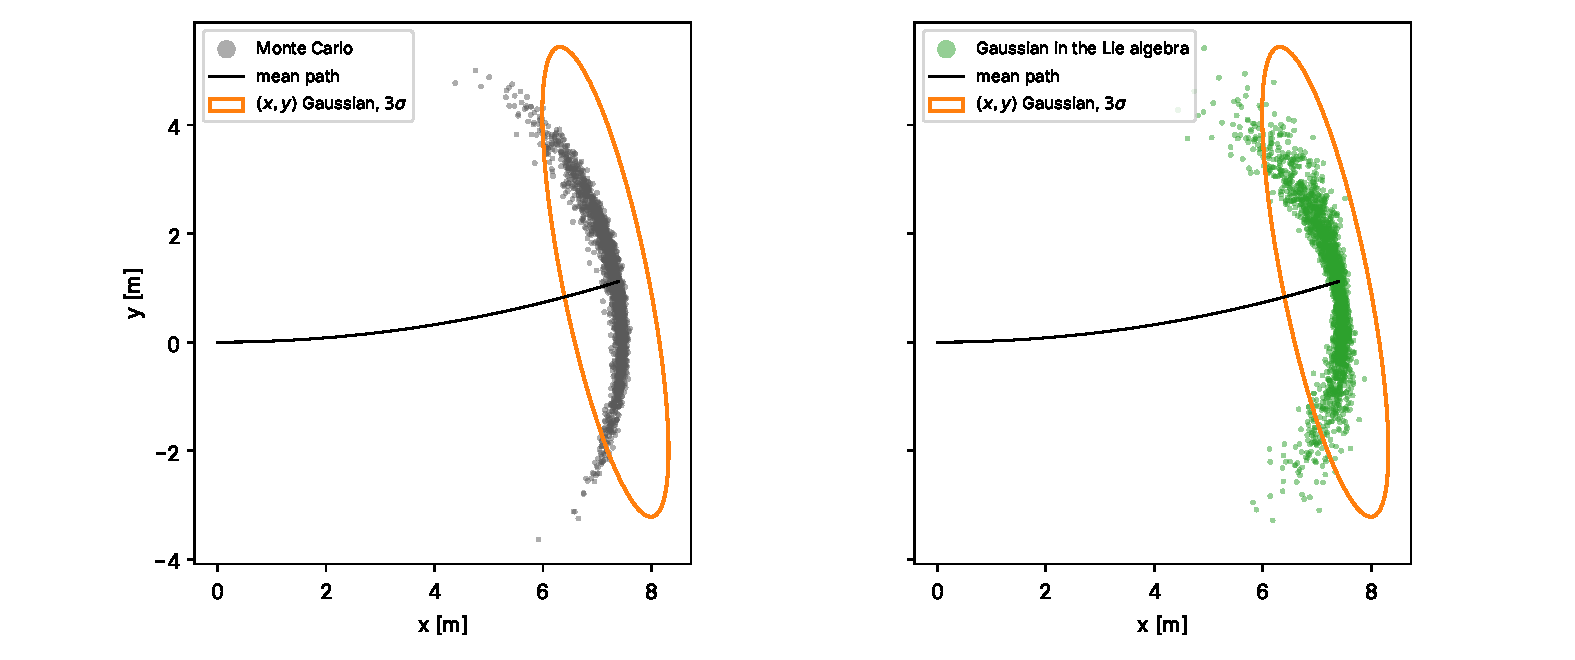
\includegraphics[width=\linewidth]{figures/ch02_banana.pdf}
\caption{Final position of the mower after $7.5$\,m of noisy odometry.
Left: Monte Carlo. Right: samples of the Lie-algebra Gaussian
propagated in closed form. The orange ellipse is the $3\sigma$ contour of
the best Gaussian in $(x,y)$: it puts probability mass where the mower
cannot be and misses the tips of the banana.}
\label{fig:banana}
\end{figure}

\begin{mower}
On a flat lawn the mower lives in $\SE2$ (Exercise~\ref{ex:se2}), and a
planar model is tempting. But gardens slope, wheels drop into ruts, and
the camera is rigidly attached to a chassis that pitches and rolls with
every bump. We therefore keep full $\SE3$ poses throughout, and add
``nearly planar'' knowledge later as a soft factor (Chapter~14), which is
exactly what the factor-graph view of Chapter~\ref{ch:slam} makes easy.
\end{mower}

\section*{Further reading and C++ pointers}
\addcontentsline{toc}{section}{Further reading and C++ pointers}

Sol\`a, Deray and Atchuthan's ``A micro Lie theory for state estimation in
robotics'' is the best short reference and uses the conventions of this
chapter; its companion C++ library is \code{manif}. Barfoot's
\emph{State Estimation for Robotics} gives the full theory with the left
convention. In C++, \code{Sophus} provides \code{SO3}/\code{SE3} with the
same tangent ordering as here and is used by many VO systems; GTSAM's
\code{Rot3}/\code{Pose3} offer the same operations with rotation-first
ordering.

\FloatBarrier
\section*{Exercises}
\addcontentsline{toc}{section}{Exercises}

\begin{enumerate}[label=\textbf{2.\arabic*},ref=2.\arabic*]
\item\label{ex:2eig} Show that the eigenvalues of $\Exp(\theta\vect{a})$
  ($\norm{\vect{a}}=1$) are $1,e^{i\theta},e^{-i\theta}$, and recover
  \eqref{eq:trace} from them.
\item\label{ex:se2} \emph{The mower's group.} $\SE2$ consists of the
  matrices $\bigl(\begin{smallmatrix}R(\theta)&\vect{t}\\\vect0\T&1
  \end{smallmatrix}\bigr)$ with $R(\theta)$ the planar rotation.
  With twist $\bxi=(\rho_1,\rho_2,\theta)$ and
  $\hatop{\bxi}=\bigl(\begin{smallmatrix}\theta\mathcal{J}&\brho\\
  \vect0\T&0\end{smallmatrix}\bigr)$, $\mathcal{J}=\bigl(
  \begin{smallmatrix}0&-1\\1&0\end{smallmatrix}\bigr)$, show that
  \[
  \Exp(\bxi)=\begin{pmatrix}R(\theta)&V(\theta)\brho\\\vect0\T&1
  \end{pmatrix},\qquad
  V(\theta)=\frac1\theta\begin{pmatrix}\sin\theta&-(1-\cos\theta)\\
  1-\cos\theta&\sin\theta\end{pmatrix}.
  \]
  Where does the mower end up after driving at $v$ for time $\tau$ with
  yaw rate $\omega$?
\item\label{ex:2cam} \emph{World to camera.} A landmark $\p_w$ is seen
  from a camera of pose $T_{wc}$; in the camera frame it is $\vect{q}=
  T_{wc}^{-1}\p_w$. Show that with a right perturbation of $T_{wc}$,
  $\partial\vect{q}/\partial\bxi=[\,-I\ \ \hatop{\vect{q}}\,]$, and that
  $\partial\vect{q}/\partial\p_w=R_{wc}\T$. This is the first half of the
  reprojection Jacobian of Chapter~3.
\item\label{ex:2adj} Show that $\Ad_T$ has determinant $1$ and is in
  general not orthogonal. What does this imply for the ``size'' of a
  covariance moved between frames?
\end{enumerate}

\subsection*{Solutions}

\textbf{2.1.} $\Exp(\theta\vect{a})\vect{a}=\vect{a}$, so $1$ is an
eigenvalue. Let $\vect{b}\perp\vect{a}$ be a unit vector and
$\vect{c}=\vect{a}\times\vect{b}$. By the In-words box after
\cref{thm:rodrigues}, in the basis $(\vect{b},\vect{c})$ of
$\vect{a}^\perp$ the rotation acts as $\bigl(\begin{smallmatrix}
\cos\theta&-\sin\theta\\\sin\theta&\cos\theta\end{smallmatrix}\bigr)$,
whose characteristic polynomial $\lambda^2-2\lambda\cos\theta+1$ has
roots $e^{\pm i\theta}$. The trace is the sum of the eigenvalues,
$1+2\cos\theta$.

\textbf{2.2.} Since $\mathcal{J}^2=-I$, the even/odd splitting of
\cref{thm:rodrigues} gives $\exp(\theta\mathcal{J})=\cos\theta\,I+
\sin\theta\,\mathcal{J}=R(\theta)$. As in \cref{thm:se3exp},
$(\hatop{\bxi})^n$ has top-right block $(\theta\mathcal{J})^{n-1}\brho$,
so the translation is $\sum_{n\ge0}\frac{(\theta\mathcal{J})^n}{(n+1)!}
\brho$. Even terms $n=2m$ contribute $\sum_m\frac{(-1)^m\theta^{2m}}
{(2m+1)!}I=\frac{\sin\theta}{\theta}I$ and odd terms $n=2m+1$
contribute $\sum_m\frac{(-1)^m\theta^{2m+1}}{(2m+2)!}\mathcal{J}=
\frac{1-\cos\theta}{\theta}\mathcal{J}$, which is $V(\theta)$. With
$\brho=(v\tau,0)$ and $\theta=\omega\tau$, the mower ends at
$\frac{v}{\omega}\bigl(\sin\omega\tau,\,1-\cos\omega\tau\bigr)$ with
heading $\omega\tau$: a circular arc of radius $v/\omega$, as expected,
and not the tangent point $(v\tau,0)$.

\textbf{2.3.} $(T\Exp(\bxi))^{-1}\p_w=\Exp(-\bxi)T^{-1}\p_w=\Exp(-\bxi)
\vect{q}\approx\vect{q}-(\brho-\hatop{\vect{q}}\bphi)$ by the computation
in the proof of \cref{prop:se3jac}(i). Hence the Jacobian
$[\,-I\ \ \hatop{\vect{q}}\,]$. The point Jacobian is the rotation part
of $T_{wc}^{-1}$, namely $R_{wc}\T$.

\textbf{2.4.} $\Ad_T$ is block upper triangular with diagonal blocks
$R$, so $\det\Ad_T=(\det R)^2=1$. It is orthogonal if and only if
$\hatop{\vect{t}}R=0$, i.e.\ $\vect{t}=\vect0$; indeed
$\Ad_T\T\Ad_T$ has top-right block $R\T\hatop{\vect{t}}R\ne0$ otherwise.
So moving a covariance between frames preserves its determinant (its
``volume'' in $\R^6$) but not its shape: rotational uncertainty is
converted into translational uncertainty proportional to the lever arm
$\norm{\vect{t}}$. This is why the uncertainty of a camera mounted far
from the mower's centre is larger than that of the body itself.
